Probabilistic latent semantic indexing\cite{hofmann1999probabilistic} is an extension to LSI which puts topic modeling under a probability framework, with which we can fit the model by maximum likelihood or Bayesian method.

\subsection{Model}
Its main idea is that each word of a document is sampled from a \emph{mixture model}, where a component is a \emph{topic} which has its own distribution with respect to the words. PLSA is also a generative model, we sample a topic variable for in each position, then the actual word is generated from the specific topic's distribution over words. 

Mathematically, PLSA models the probability of each co-ocurrence of word document pair as a mixture of conditionally independent multinomial distributions:
\begin{equation}
P(w, d) = \sum_cP(c)P(d|c)P(w|c) = P(d)\sum_cP(c|d)P(w|c)
\end{equation}
where w, d and c represents word, document and topic accordingly. This generative process can be represented in the plate notation in figure\ref{fig:plsa}.

\begin{figure}[!htbf]
\begin{center}
	\centering
	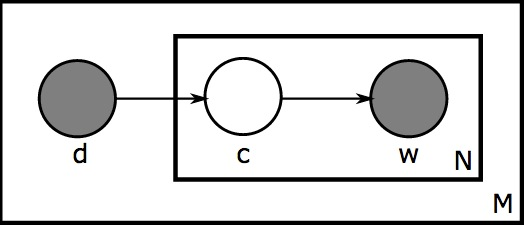
\includegraphics[width=0.8\textwidth]{FIG/plsa.png}
\caption{node plate of PLSA}
\label{fig:plsa}
\end{center}
\end{figure}



\subsection{Learning}
The Expectation-Maximization (EM) algorithm is a general algorithm for maximum-likelihood estimation where the data are incomplete or the likelihood function involves latent variables. For language modeling, the EM algorithm is often used to estimate parameters of a mixture model, in which the exact component model from which a data point is generated is hidden from us. Informally, the EM algorithm starts with randomly assigning values to all the parameters to be estimated. It then iteratively alternates between two steps, called the expectation step (i.e., the E-step) and the maximization step (i.e., the M-step), respectively. In the E-step, it computes the expected likelihood for the complete data (the so-called Q- function) where the expectation is taken w.r.t. the computed conditional distribution of the latent variables (i.e., the hidden variables) given the current settings of parameters and our observed (incomplete) data. In the M-step, it reestimates all the parameters by maximizing the Q-function. Once we have a new generation of parameter values, we can repeat the E-step and another M-step. This process continues until the likelihood converges, i.e., reaching a local maxima. Intuitively, what EM does is to iteratively augment the data by guessing the values of the hidden variables and to re-estimate the parameters by assuming that the guessed values are the true values. \cite{dempster1977maximum}
The pLSA model can be estimated using the Expectation Maximization (EM) algorithm \cite{mei2001note} to obtain the topic word distributions and the mixing weights. 

